\documentclass[main.tex]{subfiles}

\begin{document}
\chapter{Nuclear physics}

\section{Introduction}

Things to remember about nuclear units: \(\hbar c \approx \SI{197}{MeV fm} \) and \(\SI{}{MeV fm} = \SI{10}{eV \angstrom} \); there are weird things like \(e^2 = \SI{1.44}{MeV fm} \), \(4 \pi \varepsilon_0 = \). The atomic mass unit is equal to \(\SI{931.5}{MeV} \).

We have indetermination both between position and momentum: \(\Delta x \Delta p \geq \hbar/2\) and between time and energy: \(\Delta E \Delta t \geq \hbar /2\).

We can characterize the atomic particles by mass \(m\), charge \(q\), spin \(s\), half-life and mean charge radius \(\expval{\rho r^2} \sqrt{c} \): this last quantity is of the order \(\SI{.87}{fm}\) for the proton, and \(\SI{-0.1}{fm} \) for the neutron.

\section{Nuclear density}

It it roughly constant up to some radius, then it decays.
The proper way to write it would be to sum the modulus square of the wavefunction \(\psi_i\) of every nucleon:

\begin{equation}
    \rho(r) = \sum _{i} \abs{\psi_i (r)}^2
\end{equation}

We can approximate it as a radial distribution

\begin{equation}
    \rho(r) \sim \frac{\rho_0}{1 + \exp(\frac{r - r_0}{a})}
\end{equation}

where \(\rho_0 \approx 0.15 \divisionsymbol \SI{0.2}{ nucleons  \per fm^3} \) is the approximately constant density in the central region, \(r_0 \approx 1.20 \divisionsymbol \SI{1.25}{fm} A ^{1/3}  \) is the approximate radius of the nucleus (corresponding to where the density becomes half of \(\rho_0\)), \(a \approx 0.65 \divisionsymbol \SI{0.7}{fm} \) is the \emph{diffusivity}, which quantifies the length scale at which the density distribution goes to zero.

\begin{bluebox}
  Taking \(r_0 \approx \SI{1.2}{fm} \), we can estimate the nucleon density

  \begin{equation}
      \rho_0 \approx \frac{A}{V} = \frac{A}{\frac{4}{3} \pi \qty(r_0 A^{1/3})^3} \approx \SI{0.138}{fm^{-3}}
  \end{equation}

  and the corresponding mass density will be \(\approx \SI{129}{MeV \per fm^3}\) corresponding to \( \SI{2.3e17}{kg \per m^3}\), which is huge when compared to, say, that of a block of Osmium, which is around \(\SI{2.26e5}{kg \per m^3}\).
\end{bluebox}

There are also asymmetric effects, such as a skin of neutrons in the outermost part of the nucleus or a halo, which extends much further than a skin. This can be seen by looking at the differences in the scattering cross section \(\sigma \approx \pi r_0^2\).

We distinguish the nuclei by the proton number \(Z\), the neutron number \(N\) and their sum \(A = N+Z\). They are written as \(^{A} [Z]\).

\begin{itemize}
    \item Isotopes have the same \(Z\), \(^{235} \ce{U} \) and \(^{233} \ce{U}  \);
    \item Isobares have the same \(A\), \(^{44} \ce{Ca} \) and \(^{44} \ce{Ti} \);
    \item Isotones have the same \(N\), \(^{40} \ce{Ca} \) and \(^{38} \ce{Ar} \);
    \item Isomeres have the same \(Z\) and \(N\), but are in different excitation states. We require them to be somewhat stable, with half-life \({\gtrsim \SI{e-12}{s}}\), \(^{99}\ce{Tc}  \) and \(^{99m}\ce{Tc}  \).
\end{itemize}

We also define specular nuclei: denoting the nuclear numbers as \((N,Z)\), \((a, b)\) is isobaric and specular to \((b, a)\).

\begin{bluebox}
  At the driplines, the excess nucleons are not bound (the effective potential they are in does not have a minimum).

  \(^{8} \ce{B} \) and \(^{8} \ce{Be} \) are isobares.

  \(^{19} \ce{F} \) is an isotone to \(^{17} \ce{F} \).

  The stable isotopes of Samarium are those with \(A=144\), 150, 152, 154.

  The specular nuclide to \(^{11} \ce{Li} \) would be \(^{11} \ce{O} \), but it does not seem to exist.
\end{bluebox}

The mass of a nuclide is given by

\begin{equation}
M (A, Z) = Z m_p + (A-Z) m_n - B(A, Z)
\end{equation}

 where \(B\) is the binding energy. It is a good first approximation to say \(B/A \approx \text{const}\), around \(\SI{8}{MeV} \).

Actually, this value increases up to iron, then very slowly decreases, with slight bumps at magic numbers.

\section{Waterdrop model}

A nucleus is similar to a water droplet, like:

\begin{itemize}
    \item \(\nabla \cdot \vec{v} = 0  \) and similarly the nucleons are roughly incompressible, mantaining a constant density inside the nucleus;
    \item The evaporation heat of a water drop is directly proportional to its mass, and similarly we can approximate \(B \propto A\);
    \item The water molecules are held together by intermolecular Van der Waals forces, with expressions like \(r ^{-12} - r ^{-6} \), and similarly the strong nuclear force has a short range.
\end{itemize}

We can write a Semi Empiric Mass Formula, which will give us  the best estimate of the waterdrop model for the nuclear mass. We will assume that the nuclear forces \emph{saturate} after a certain point, that is, they have finite support.

\paragraph{Volume term}

The full potential is

\begin{equation} \label{eq:waterdrop-volume-full-potential}
    V = \sum _{i<j} V_{ij} (\abs{r_i - r_j})
\end{equation}

so if the nuclear force was long-range we would have \(B \propto A (A-1) \expval{V} \), since the terms in the sum \eqref{eq:waterdrop-volume-full-potential}  are \(A(A-1)/2\) (by \(\expval{V} \) I mean the average binding energy in a nucleon pair).

We must account for the fact that the nucleons only interact with their neighbours in some fixed volume \(V_ \text{int}\): so

\begin{equation}
    B \propto \frac{A(A-1) V _ \text{int}}{ \underbrace{V_\text{total}}_{\substack{\propto A}} } \propto A-1 \sim A
\end{equation}

So our first term will be

\begin{equation}
    B \sim a_V A
\end{equation}

\paragraph{Surface term}

The surface nucleons interact with less nucleons than the internal ones. This effect will surely be negative and proportional to the surface area, and we are only interested in proportionality, so

\begin{equation}
    B \sim a_V A - a_S A ^{2/3}
\end{equation}

\paragraph{Coulomb term}

The positively charged nucleons repel each other: we model the nucleus as a uniformly charged sphere, which will have charge density \(\rho = 3Ze / \qty(4 \pi R^3)\), where \(R\) is the radius of the nucleus. Applying \(\nabla \cdot E = \rho/ \varepsilon_0\) and integrating over a sphere of radius \(r\), we get

\begin{equation}
    E(r) = \begin{cases}
        \frac{Zer}{4 \pi \varepsilon_0 R^3 } = \frac{\rho r}{4 \varepsilon_0} \qquad r \leq R  \\
        \frac{Ze}{4 \pi \varepsilon_0 r^2} = \frac{\rho R^3}{3 \varepsilon r^2} \qquad r \geq R
\end{cases}
\end{equation}

The energy density of the electric field is given by \(u = \varepsilon_0 E^2/2\); its integral over all of  space \(U = 4 \pi \int _{0}   ^{\infty} ur^2\dd{r}   \), which corresponds to the Coulomb term to subtract to the binding energy, can be calculated analytically, and is the sum of the external and internal contributions:

\begin{equation}
    U = \qty(1 + \frac{1}{5}) \frac{(Ze)^2}{8 \pi \varepsilon R}
\end{equation}

Then we can put all the constants into a term, leaving out only the proportionalities to \(Z^2\) and \(R^{-1} \propto A^{-1/3}\). Now our formula is:

\begin{equation}
    B \sim a_V A - a_S A ^{2/3} - a_C Z^2 A ^{-1/3}
\end{equation}

with

\begin{equation}
    a_C = \frac{3}{5} \frac{e^2}{4 \pi \varepsilon_0} \frac{1}{r_0} \approx \SI{0.7}{MeV}
\end{equation}

which can be found by recalling \(e^2 = e^2 / (4 \pi \varepsilon_0) \approx \SI{1.44}{MeV fm} \) and \(r_0 \approx 1.2 \divisionsymbol \SI{1.3}{fm} \).

It might be more accurate for this term to be proportional to \(Z(Z-1)\), since the proper expression for the energy will be:

\begin{equation} \label{eq:SEMF-coulomb-correction}
    U = \frac{e^2}{4 \pi \varepsilon_0} \sum _{i=1}   ^{Z} \sum _{j<i} \frac{1}{\abs{r_i - r_j} }  \propto \frac{Z(Z-1)}{\abs{\overline{r} } }  \propto \frac{Z(Z-1)}{A^{1/3}}
\end{equation}

where \(\overline{r} \) is the average distance between the protons in the nucleus. We do not know what it looks like, but surely \(\overline{r} \propto r _{\text{nucleus}}  \propto A^{1/3}\).

\paragraph{Asymmetry term}

The binding energy between \(pp\) is similar to that between \(nn\), let us call it \(v\), but it is smaller than the \(pn\) attraction by a factor \(\sim 2\), so let us call the \(np\) energy \(2v\). This can be seen empirically from the fact that \(nn\) and \(pp\) are not bound states, while the deuton (\(^{2} \ce{H} \)) is.
The factor is around 2 because of the Pauli exclusion principle: nucleons are spin\(-1/2\) fermions, so if their spins and isospins are the same they cannot come near one another: the spins will be aligned around half of the times that the isospins are aligned, so this justifies the factor of 2.

The asymmetry term becomes relevant for large \(A\).

When counting the total binding energy we must divide by \(A\) to account for the fact that every nucleon only interacts with its neighbours.

\begin{subequations}
\begin{align}
    B _A
    &= \frac{N v}{A} \qty(N + 2 P)  + \frac{P v}{A} \qty(2N + P) \\
    &= \frac{v}{A} \qty(N^2 + P^2 + 4 NP)  \\
    &= \frac{v}{2A} \qty(3N^2 + 3P^2 + 6NP - N^2 - P^2 + 2NP) \\
    &= \frac{v}{2A} \qty(3A^2 - (N-Z)^2)
\end{align}
\end{subequations}

The linear term in \(A\) is the volumetric term; the term to add is \(\propto (N-Z)^2 / A\). So now we have

\begin{equation}
    B \sim a_V A - a_S A ^{2/3} - a_C Z^2 A ^{-1/3} - a_A \frac{(N-Z)^2}{A}
\end{equation}

This can be also seen by approximating the nucleus as a Fermi sea: if \(N=Z\) all the nucleons can be at the Fermi energy \(\varepsilon_F\), while if there is a difference some of them will have more energy.

Take \(N-Z = 4i\), with \(i \in \N\), and imagine moving to this configuration from \(i=0\). The first two protons becoming neutrons will raise the energy of the nucleus by \(2 \Delta E\), where \(\Delta E\) is the separation between the energy levels. The next step will take \(6 \Delta E\), and in general  the \(j+1\)-th will take \(2 (2j+1) \Delta E\): we need to add these up,

\begin{equation}
    \sum _{j=1} ^{i} 2 (2j+1) \Delta E =   2 i^2 \Delta E = 2\frac{(N-Z)^2}{16} \Delta E
\end{equation}

It can also be shown (CHECK LATER) that \(\Delta E \propto 1/A\). Then we get the same formula as before.

\paragraph{Pairing term}

It is added to the formula to explain the experimental data: the term we need to add looks like

\begin{equation}
    B_P = \frac{a_P}{A^{1/2}} \qquad a_P = \begin{cases}
        + \delta \quad &\text{even-even}  \\
        0 \quad &\text{even-odd}  \\
        - \delta \quad &\text{odd-odd}
\end{cases}
\end{equation}

with \(\delta \sim 11 \divisionsymbol \SI{12}{MeV} \). It is due to the wavefunctions of the nuclides ``pairing up'' in some sense. The exponent being 1/2 is not certain, some say 3/4 fits the data better\dots

\paragraph{SEMF}

The full formula looks like

\begin{equation} \label{eq:SEMF}
    B \sim a_V A - a_S A ^{2/3} - a_C Z^2 A ^{-1/3} - a_A \frac{(N-Z)^2}{A} \pm \frac{a_P}{A^{1/2}}
\end{equation}

with \(a_V \approx \SI{16}{MeV} \), \(a_S \approx \SI{17}{MeV} \), \(a_C \approx \SI{0.7}{MeV} \), \(a_A \approx \SI{23}{MeV} \), \(a_P \approx \SI{12}{MeV} \). It fits the data well, for \(A>10 \divisionsymbol 20\).

The empirical data do not exactly follow the SEMF: the binding energy is slightly higher at certain \emph{magic numbers}.

The highest binding energy per nucleon is found with \(^{62} \ce{Ni} \) (\(B/A = \SI{8.7945}{MeV} \)), while the lowest mass per nucleon is found with \(^{56} \ce{Fe} \). They can be different because they have different proton/neutron ratios.

\paragraph{Mass parables}

If we work at fixed \(A\), the \eqref{eq:SEMF} looks like a parabola wrt \(Z\). Actually, if \(A\) is even it looks like two parabolas, distanced \(2\delta\) apart, with the nuclides switching from one to the other as the parity of \(Z\) changes; if \(A\) is odd the nuclides are always even-odd so it is just one parabola. The asymmetry term is proportional to \((A-2Z)^2\), so we get:

\begin{equation} \label{eq:mass-parabola-params}
    B = Z^2 \qty(-a_C A^{-1/3} - \frac{4 a_A}{A}) + Z\qty(4a_A) + \text{const}
\end{equation}

\begin{bluebox}
  We perform a parabolic fit for the nuclei at \(A = 148\), and compute the coefficients corresponding to the fit parameters according to formula \eqref{eq:mass-parabola-params}. The results are shown in \ref{fig:mass-parabola-fit}.

  The fit parameters give \(a_A = \SI{21.41}{MeV}\), \(a_C = \SI{0.65}{MeV}\), \(a_P = \SI{12.26}{MeV}\). The energy at the vertex of the parabola can be calculated from the model assuming \(a_V = \SI{16}{MeV}\) and \(a_S = \SI{17}{MeV}\) to be \SI{1340}{MeV}, while the real energy is  \SI{1225}{MeV}.
\end{bluebox}

\begin{figure}[H]
  \centering
  \begin{subfigure}{0.5\textwidth}
      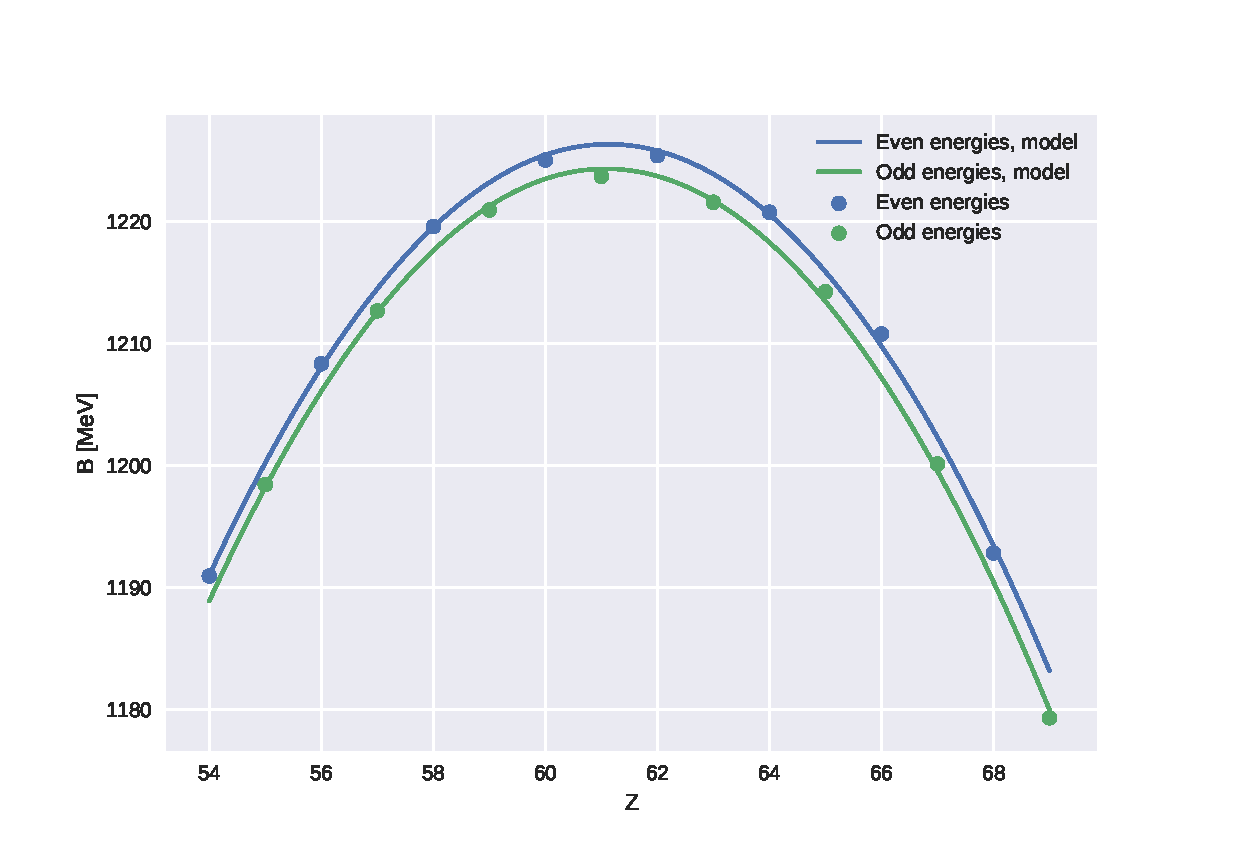
\includegraphics[width=\textwidth]{figures/parabolic_fits.eps}
      \caption{Fit and raw data}
  \end{subfigure}%
  \begin{subfigure}{0.5\textwidth}
      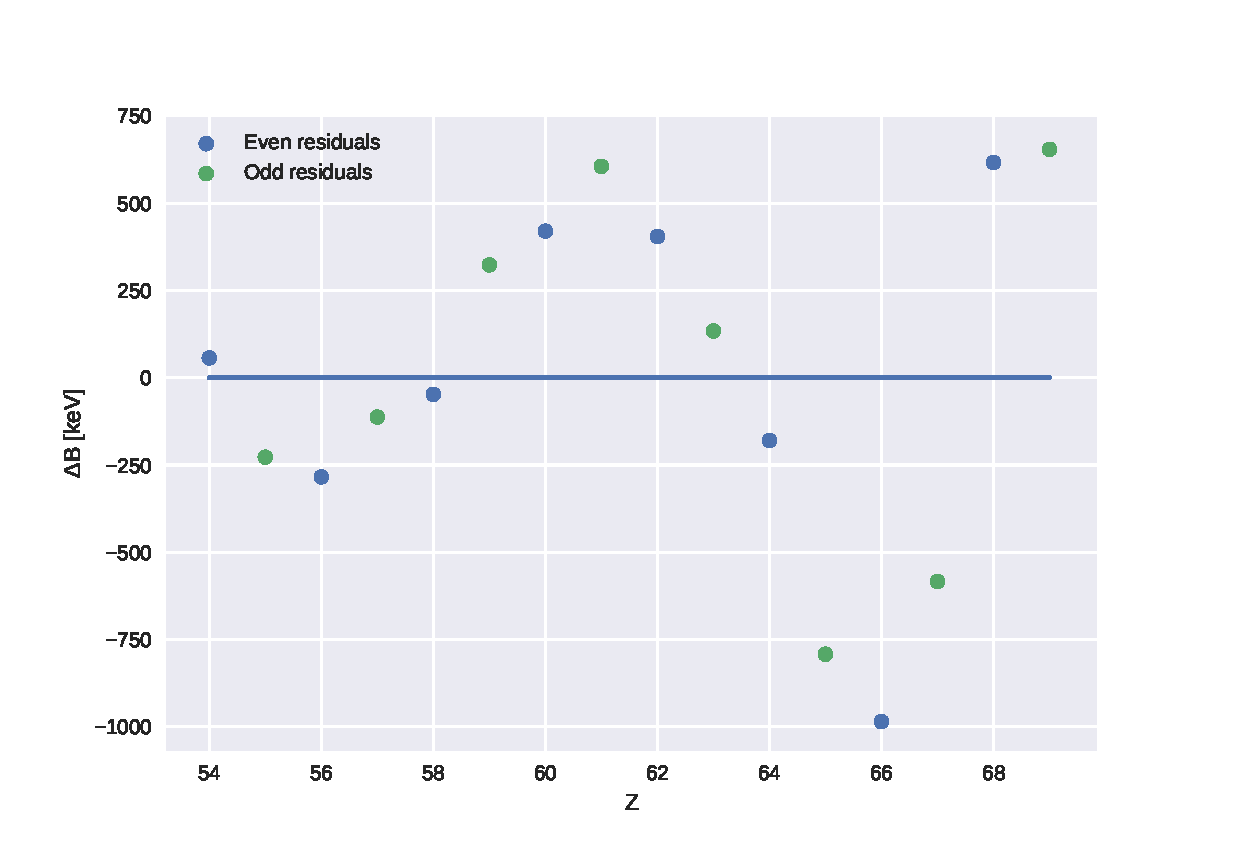
\includegraphics[width=\textwidth]{figures/residuals.eps}
      \caption{Residuals of the fit}
  \end{subfigure}
  \caption{Mass parabola fit}
  \label{fig:mass-parabola-fit}
\end{figure}

There are some odd-odd stable nuclei, like \(^{14} \ce{N} \), but they are rare.

\paragraph{Specular nuclei}

If they have \(\Delta Z = 1\) and \(A\) is odd, interesting things happen. Our working example is \(^{15} _{8   } \ce{O} _{7} \) and \(^{15} _{7} \ce{N}_8 \).

The only term which changes in the SEMF between them is the Coulomb term: their \(Z\)s are \((A \pm 1)/2\), therefore (applying the corrected Coulomb formula given in \eqref{eq:SEMF-coulomb-correction}) their difference in energy is given by

\begin{subequations}
\begin{align}
  \Delta B  &= \frac{a_C}{A^{1/3}} \qty(\frac{(A+1)(A-1)}{4} - \frac{(A-1)(A-3)}{4})  \\
  &= \frac{a_C}{A^{1/3}} \qty(\frac{4A -4}{4})  \\
  &= a_C \qty(A^{2/3} - A^{-1/3})
\end{align}
\end{subequations}

We can plot the data for \(\Delta B\) wrt \(x \defeq A^{2/3}\). The plot will be of the form

\begin{equation}
    \Delta B  = a_C x - \frac{a_C}{\sqrt{x}}
\end{equation}

The fit works, giving us \(a_C = \SI{631(5)}{keV}\) in this parametrization.

\begin{figure}[H]
    \centering
    \begin{subfigure}{0.5\textwidth}
        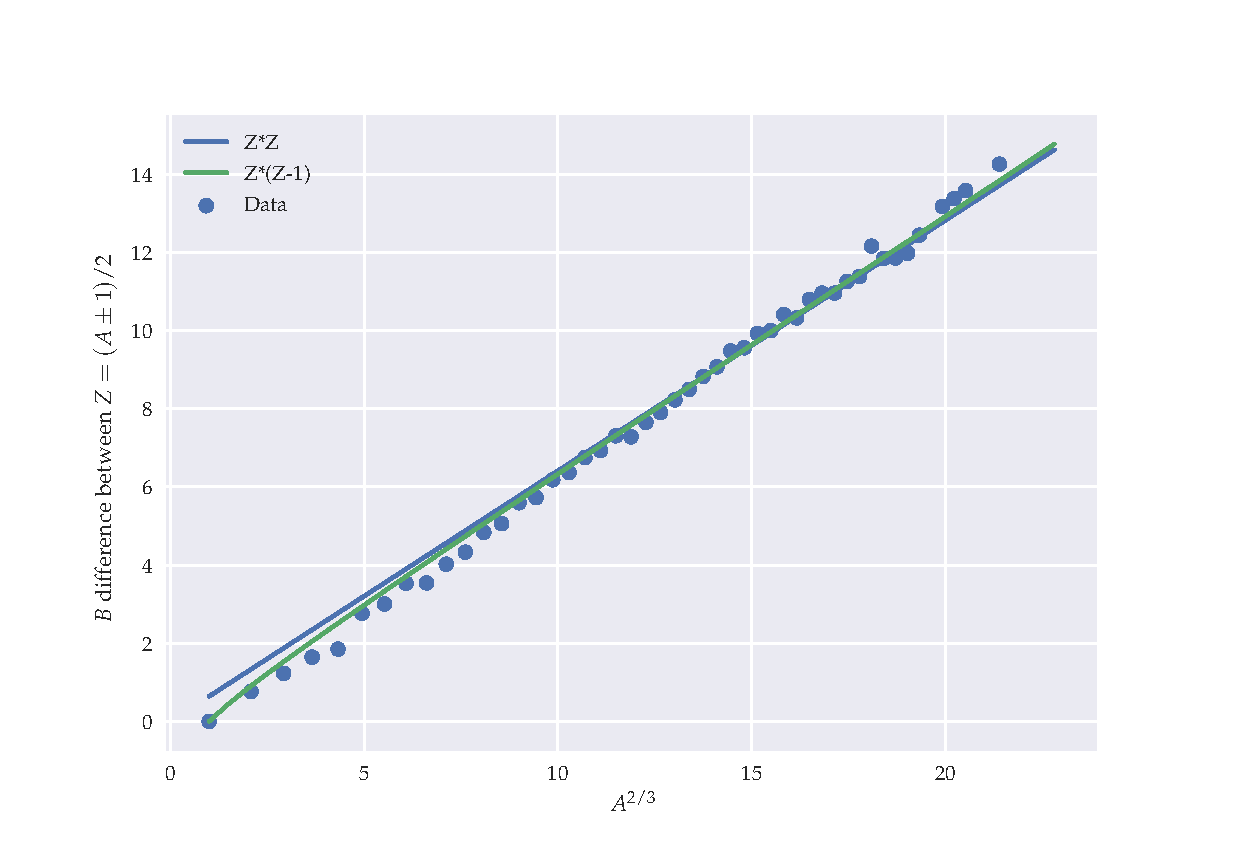
\includegraphics[width=\textwidth]{figures/odd_A_fit.eps}
        \caption{Fit}
    \end{subfigure}%
    \begin{subfigure}{0.5\textwidth}
        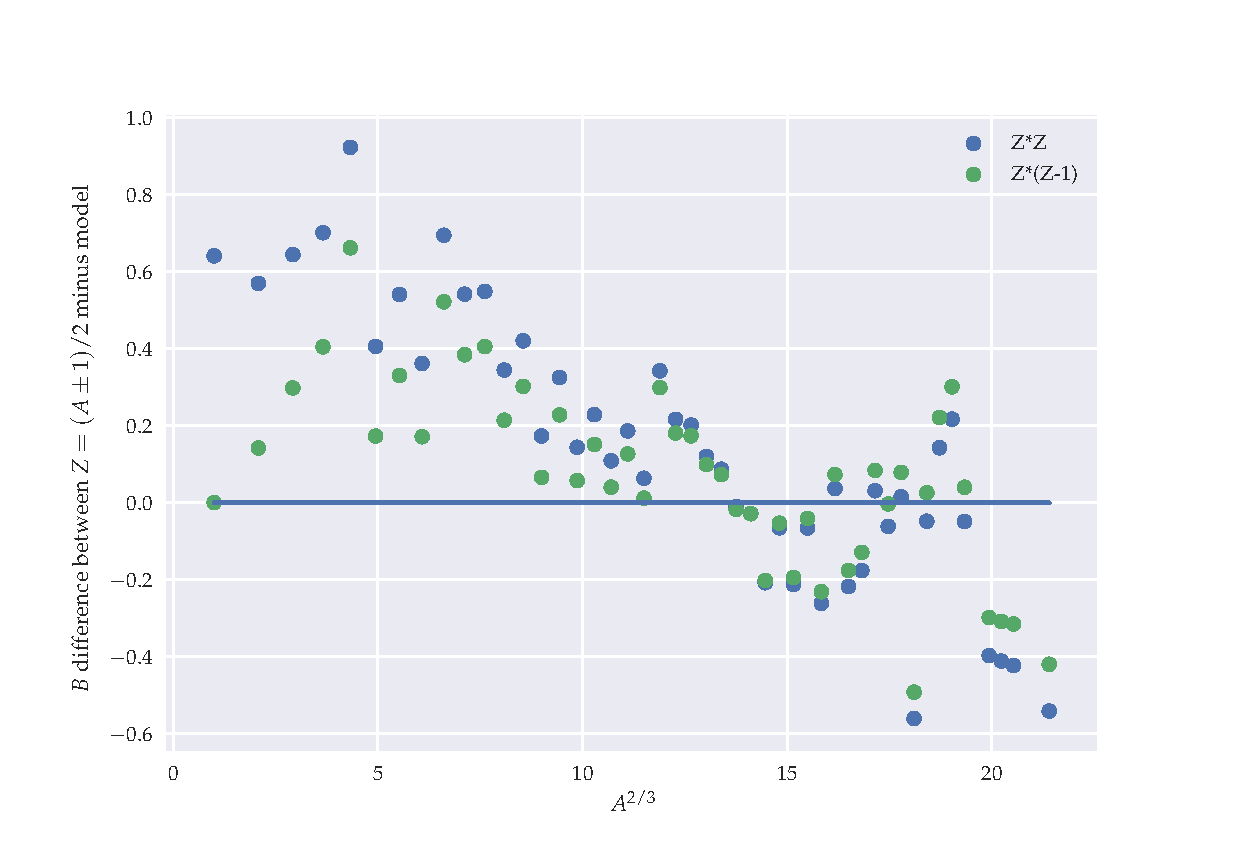
\includegraphics[width=\textwidth]{figures/odd_A_residuals.eps}
        \caption{Residuals}
    \end{subfigure}%
    \caption{Fit of the difference in \(B\) between symmetric nuclei. The chi square is \(\SI{0.136}{MeV^2} \) for the \(Z^2\) model, and \(\SI{0.062}{MeV^2}\) for the \(Z(Z-1)\) model.}
    \label{fig:odd-A-fit}
\end{figure}

\section{Fermi gas model}

\paragraph{Hypotheses}

\begin{itemize}
    \item The nucleons are spin \(1/2\) fermions;
    \item the nucleons' collective actions can be represented with a spherically symmetric potential well \(U(r)\), extended in a radius \(R = r_0 A^{1/3}\);
    \item the nucleon gas is degenerate: the kinetic energy of the nucleons is much less than the thermal energy \(k_B T\).
\end{itemize}

The proper Hamiltonian, without the mean-field approximation,  would be

\begin{equation}
    H = \sum _{i} T_i + \sum _{i<j} V_{ij} \qty(\abs{r_i - r_j} )
\end{equation}

instead, we use

\begin{equation}
    H_{\text{sp}} = -\frac{\hbar^2 \nabla^2}{2 \mu} + U(r)
\end{equation}

where \(\text{sp}\) means 'single particle', \(\mu ^{-1} = m _{\text{sp}} ^{-1} + m _{\text{nucleus}} ^{-1}\).

For nuclei at human temperatures, \(\lesssim \SI{e3}{K} \), we have energies \(\lesssim \frac{3}{2} k_B T = \SI{0.13}{eV}  \ll MeV \), so thermal motion is negligible.

\paragraph{\(1D\) infinite well}

We have an infinite well from \(-a/2\) to \(a/2\), and inside it a particle of mass \(m\).

The solutions to the time-independent Schrödinger equation are in the form

\begin{equation}
    \psi(x) = A \sin(kx) +B \cos(kx)
\end{equation}

where \(k^2  = 2mE / \hbar^2\) is the square of the wavenumber, which is directly proportional to the momentum \(k = p/\hbar = 2 \pi / \lambda\). We must also consider the boundary conditions: the domain of the Hamiltonian is \(\qty{\psi(x) \in L^2 \,|\, \psi(\pm a/2)=0 } \).

So we have two classes of solutions, proportional to either \(\cos((2q)\pi x/a)\) or \(\sin((2q+1)\pi x/a)\) with \(n
\in \N\). If we call the even or odd number \(2q (+1) = n_x\), the energy comes out to be

\begin{equation}
    E = \frac{\hbar^2 k^2}{2m} = \frac{h^2 n_x^2}{8ma^2}
\end{equation}

\paragraph{\(3D\) potential well}

The problem works out analogously, with

\begin{equation}
    E = \frac{h^2}{8ma^2} \sum _i  n_i^2
\end{equation}

so we work in the space \(\Z_+^3 \ni \vec{n} \), where same-energy states live in spherical shells.

The differential number of states in these shells is (approximately) given by the volume of the shell, which is an eighth of the sphere's: \(N = \frac{1}{8} 4 \pi n^2 \dd{n} \). This can also be written as \(\rho(E) \dd{E} \), that is, it corresponds to a density of states.

Then, since the energy is just a function of \(n\), we have

\begin{equation}
    \dd{E} = \frac{h^2}{8ma^2} \dd{(n^2)} =   \frac{h^2}{4ma^2} n\dd{n}
\end{equation}

Therefore we can substitute in:

\begin{equation}
    \rho(E) \dd{E} = \frac{\pi}{2} \underbrace{n}_{\substack{\sqrt{8ma^2 E/h^2}}} \underbrace{n \dd{n} }_{\substack{4ma^2 / h^2} \dd{E} } = \frac{2 \pi  \qty(2ma^2)^{3/2}}{h^3} \sqrt{E} \dd{E}
\end{equation}

and we can also express this wrt \(p = \sqrt{2mE} \); its differential is \(p\dd{p} = m \dd{E} \):

\begin{equation} \label{eq:fermi-model-momentum-density}
    \rho(E) \dd{E} = \rho(p) \dd{p} = V \frac{4 \pi a^3 p^2 \dd{p} }{h^3}
\end{equation}

Where \(a^3 = V\) is the volume, and since we treat a spherically symmetric problem we can rewrite it as \(V = \frac{4}{3}\pi r_0^3\). Then, we put two fermions in each shell, thus getting \(N\) particles in total; multiplying by \(A\) since there are \(A\) nucleons in total and our pdf is normalized for 1 particle.

\begin{equation} \label{eq:fermi-state-density}
    \dd{N} = 2 \rho(p) \dd{p} = \frac{4}{3 \pi} \frac{r_0^3 p^2}{\hbar^3} A \dd{p}
\end{equation}

\paragraph{Fermi sea}

This probability density must be normalized: let us consider the protons first. If their occupation is maximal up to \(p_F\) and null after, it must be

\begin{equation}
    Z
    = \int _{0}  ^{p_F} 2 \rho( p)  \dd{p}
    = \int _{0}  ^{p_F} \frac{4}{3 \pi} \frac{r_0^3 p^2}{\hbar^3} A \dd{p}
    = \frac{4 A}{9 \pi} \frac{r_0^3 p_F^3}{\hbar^3}
\end{equation}

Turning this around gives

\begin{equation} \label{eq:fermi-sea-momentum-protons}
    p_F c = \frac{\hbar c}{r_0} \sqrt[3]{\frac{9 \pi }{8} \frac{2Z}{A}}
\end{equation}

and we can find a similar result for the neutrons.
Note that, if the nucleus is close to being symmetric, \(p_F\) only depends on \(r_0 \propto \rho_0 = A/V\), not on \(A\) or \(V\) re

For light nucluei we can assume \(2Z/A \approx 1\), and we know that \(r_0 \approx \SI{1.25}{fm} \). Then \(p_F \approx \SI{240}{MeV/c} \) and \(E_F \approx \SI{31}{MeV/c^2} \)

If we assume that \(V = E_F + B/A\) (as in, if we were to remove one nucleon at a time we would on average find them at the energy \(-B/A\)) we find that the potential well is around \(\SI{40}{MeV}\) deep.

One more prediction of this model is that, for heavy nuclei with \(N>Z\), \(E_{F_N} > E_{F_P}\); the magnitude of the difference is around \(32\) vs \(\SI{28}{MeV} \) for Uranium.

\paragraph{Isospin}

We consider nucleons as different manifestations of a single particle, with different eigenvalues for the \(z\) component of an operator \(\vec{T} \), which has algebra \(\mathfrak{su}(2)\). So, we assume that the nucleon is an isospin-\(1/2\) particle (that is, the eigenvalue of \(T^2\) is \(3\hbar^2 /4 = \hbar^2 i (i+1)\)).

\paragraph{Average kinetic energy}

We have computed the state distribution differential \(\dd{N} \), with \(\int   \dd{N}  = A\) in equation \eqref{eq:fermi-state-density}. It is useful to split the neutron and proton contributions since in heavy nuclei their numbers differ significantly.
For both of them we can find:

\begin{equation}
    \expval{E_k}
    = \frac{1}{A} \int _{0}   ^{A} p^2 /(2m) \dd{N}
    = \frac{1}{A} \int _{0}   ^{p_F} \frac{p^2}{2m} \frac{4}{3 \pi} \frac{r_0^3 p^2}{\hbar^3} A \dd{p}
    = \frac{4}{3 \pi} \frac{r_0^3 }{\hbar^3} \int _{0}   ^{p_F} \frac{p^4}{2m} \dd{p}
\end{equation}

so adding their contributions we get

\begin{equation}
    \expval{E_k} = \frac{4 r_0^3}{3 \pi \hbar^3} \qty(\frac{p_{F_p}^5}{10 m_p} + \frac{p_{F_n}^5}{10 m_n})
\end{equation}

and we can substitute in the formula for the Fermi momentum \eqref{eq:fermi-sea-momentum-protons}, and approximate \(m \approx  m_n \approx  m_p\): we get

\begin{subequations}
\begin{align}
    \expval{E_k}
    &= \frac{4 r_0^3}{30 m \pi \hbar^3} \qty(\qty(\frac{\hbar}{r_0} \sqrt[3]{\frac{9 \pi }{8} \frac{2Z}{A}})^5 + \qty(\frac{\hbar}{r_0} \sqrt[3]{\frac{9 \pi }{8} \frac{2(A-Z)}{A}})^5)  \\
    &= \frac{3^{7/3}}{80} \frac{\pi^{2/3} \hbar^2}{80 Am r_0^2} \qty(\qty(\frac{2Z}{A})^{5/3} + \qty(\frac{2(A-Z)}{A})^{5/3})
\end{align}
\end{subequations}

Now, \(2Z/A\) is approximately 1, so we can do a series expansion! \(2Z/A \approx 1+x\), where \(x = (2Z-A)/A\).

We can use \((1+x)^{5/3} + (1-x)^{5/3} = 2 + 10x^2/9 + O(x^3)\). So,

\begin{equation}
    \expval{E_k} =  \frac{3^{7/3}}{80} \frac{\pi^{2/3} \hbar^2}{40 Am r_0^2} \qty(1 + \frac{5}{9} \qty(\frac{2Z-A}{A})^2)
\end{equation}

\section{Nuclear fission}

\paragraph{Ellipsoid deformations}

The nucleus is approximately spherical, but we can model its oscillations as having an axis of rotational symmetry, thus having the shape of an ellipsoid. We call its two equal axes \(b\) and its different axis \(a\). If \(a>b\) the ellipsoid is prolate, otherwise it is oblate.

Since the volume is conserved, if \(R=a=b\) is the spherical configuration, a small perturbation of it must look like \(a = R(1+ \varepsilon )\), \(b = R(1+\varepsilon)^{-1/2}\).

Calculations show that the surface increases like \( 4 \pi R^2 \rightarrow 4 \pi R^2 \qty(1  + (2/5) \varepsilon^2 + O(\varepsilon^3))\), therefore \(A^{2/3} \rightarrow \qty(1+ (2/5)\varepsilon^2) A^{2/3}\); we will also need the fact that \(A^{-1/3} \rightarrow \qty(1-(1/5)\varepsilon^2) A^{-1/3}\).

The part of the SEMF that changes looks like

\begin{equation}
    B = - a_S A^{2/3} - a_C \frac{Z^2}{A^{1/3}} +  \text{const}
    \rightarrow - a_S A^{2/3} \qty(1+ \frac 25 \varepsilon^2)  - a_C \frac{Z^2}{A^{1/3}} \qty(1-\frac 15 \varepsilon^2)+  \text{const}
\end{equation}

so we can compute the difference \(B_ \text{new} - B _ \text{old} = \Delta B\):

\begin{equation}
    \Delta B
    = A^{2/3} \qty( - a_S  \frac 25 \varepsilon^2 + a_C \frac{Z^2}{A} \frac 15 \varepsilon^2)
    = A^{2/3} \frac{\varepsilon^2}{5} \qty(-2a_S + a_C \frac{Z^2}{A})
\end{equation}

this changes sign, becoming positive, for \(a_S / a_C < Z^2 / (2A)\). The ratio of the constants is known and approximately equal to \(2a_S /a_C \approx 49\). At that point, becoming more elliptical corresponds to gaining energy, so the nucleus is unstable and will fission.

The inequality is reached around \(Z \approx 114\), \(A \approx 270\). This is not the limit seen experimentally: nuclei fission as early as \(Z^2 / A \approx 35\), but it gives a good theoretical justification of the fact that after a certain point we do not find any more stable nuclei.

\paragraph{Nuclear fission}

\(^{235, 238}\ce{U} \) fission spontaneously, around \(\SI{e-9}{}\) to \(\SI{e-5}{} \) of the times they alpha-decay.

In fisssion from \(^{238} \ce{U} \) to \(A \approx 119\) nuclei around \(\SI{200}{MeV} \) of energy is emitted.

\paragraph{Neutron capture causing change in \(Z\)}

It works like this: the atom (say, \(^{238} \ce{U} \)) absorbs a neutron, becoming the excited \(^{239*} \ce{U} \); then, this nucleus emits gamma radiation becoming \(^{239} \ce{U} \), finally it balances the neutron excess by decaying \(\beta^-\) and thus becoming \(^{239} \ce{Np} \).

\paragraph{Neutron capture causing fission}

The capture of a neutron can make an atom unstable wrt deformation, and then it might tunnel through the potential barrier.

\begin{figure}
    \centering
    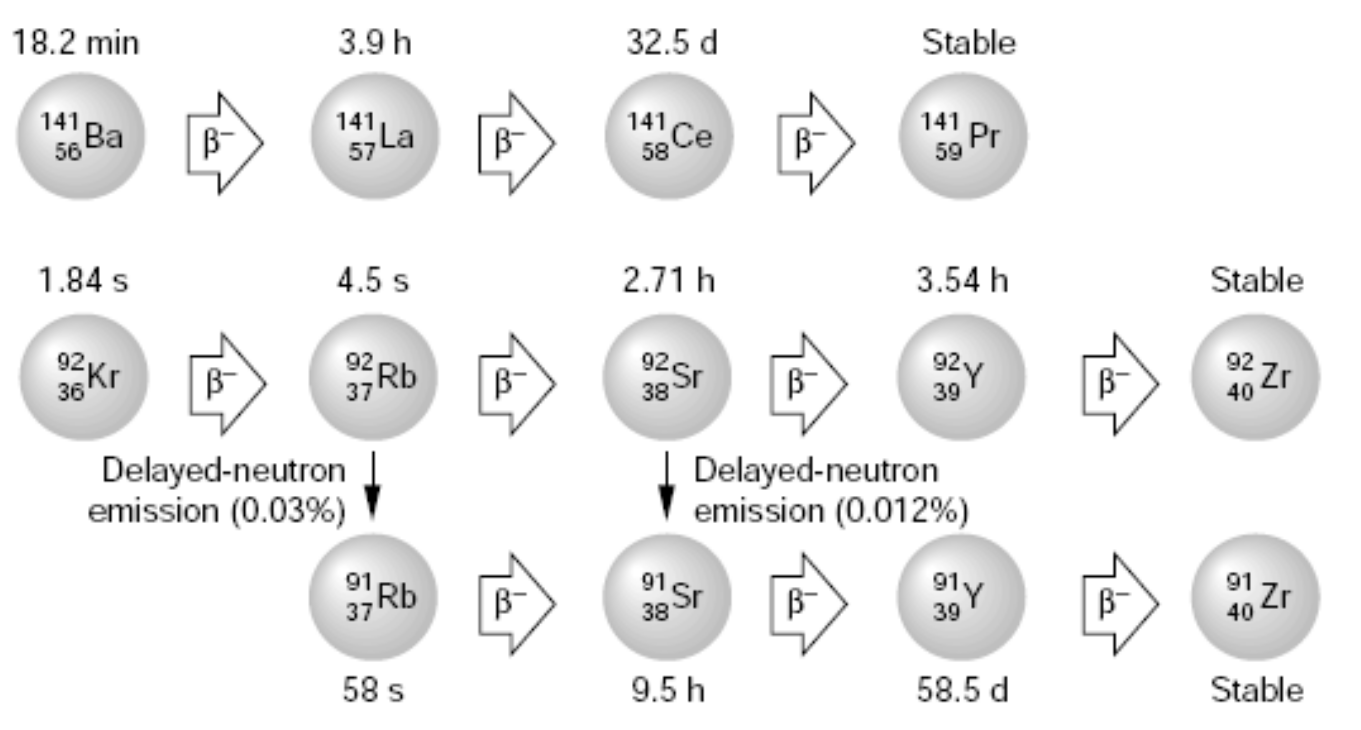
\includegraphics[width=0.7\textwidth]{figures/barium_decay_chain.png}
    \caption{Barium decay chain}
    \label{fig:barium-decay}
\end{figure}

Since the \(N/Z\) ratio is higher in heavier nuclei, the fission products will not be stable with the amount of neutrons they end up with, so they will tend to emit neutrons.

Some atoms have low energy barriers for fission, which can be surpassed by ambient temperature neutrons with \(E = k_B T_ \text{amb} \approx \SI{26}{meV} \) (\(^{235} \ce{U} \) is like this), while others need fast-moving neutrons (like \(^{238} \ce{U} \)).

The probability of a nucleus of mass \(A\) being emitted in symmetric nuclear fission is bimodal, with high regions around \(A \approx 90\) and \(A \approx 130\).

\section{Nuclear Fusion}

Nuclear fission reactions can have very high energy yields,  but also have high activation energies because of the Coulomb barrier.

\begin{equation}
    Q = - \sum _ \text{reagents} E_i + \sum _{\text{products}} E_i
\end{equation}

Between the first nuclear fusion reactions one can write, the highest in \(Q\) is \(\ce{d}+\ce{d} \rightarrow ^{4} \ce{He} + \gamma\) with \(Q  \approx  \SI{24}{MeV} \), while other reactions with protons and deutons have \(Q = 3 \divisionsymbol \SI{5}{MeV} \).

\paragraph{Coulomb barrier}

Its height is

\begin{equation}
    V_C = \frac{e^2}{4 \pi \varepsilon_0} \frac{Z_1 Z_2}{R}
\end{equation}

where \(R\) is the sum of the radii of the nuclei, a distance at which we assume the nuclear forces take over. For example, in the \(\ce{d} + \ce{d}\) reaction, \(V_C \approx \SI{500}{keV} \).

\begin{figure}[H]
    \centering
    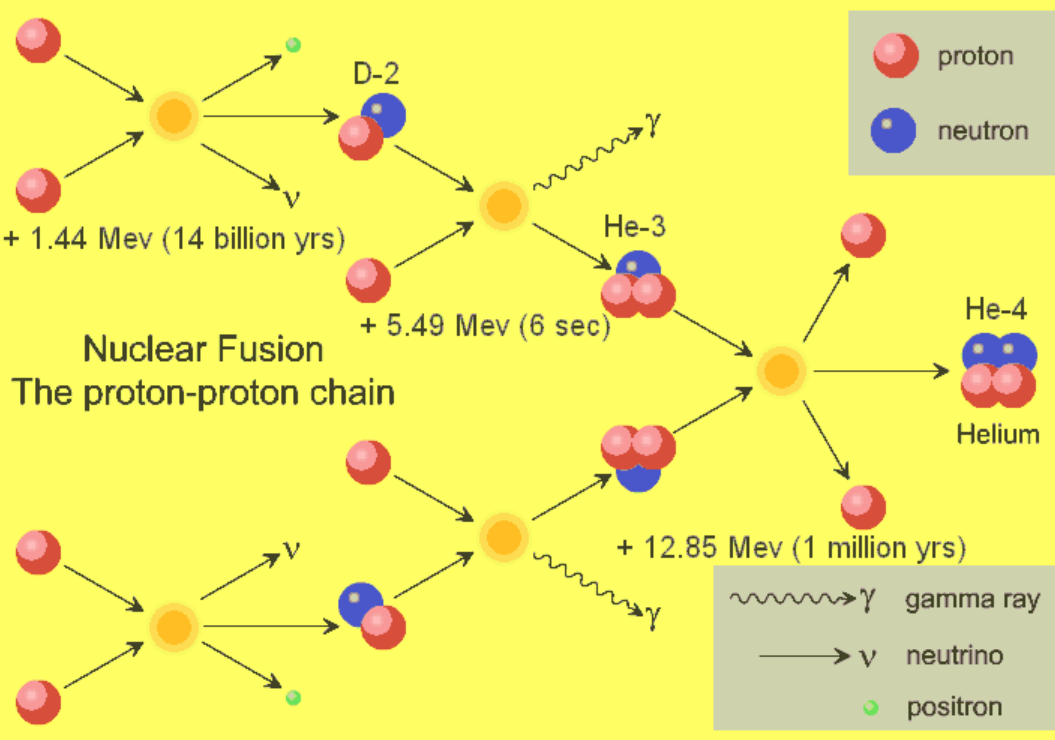
\includegraphics[width=0.7\textwidth]{figures/sun_nuclear_fusion.png}
    \caption{Nuclear decay chain in the Sun.}
    \label{fig:nuclear-fusion-sun}
\end{figure}

In figure \ref{fig:nuclear-fusion-sun} we show the nuclear fusion chain in the sun: from just protons we get \(^{4} \ce{He} \), with a release of \(\SI{26.73}{MeV} \).

To get a high yield in nuclear fusion we need a kinetic energy on the order of \(\SI{10}{keV} \), which corresponds to very high temperatures.

\section{Deuton}

It is the only two-nucleon bound state; it has a \emph{total}  energy of \(\SI{2.224}{MeV} \)

Its rms radius is around \(\SI{2}{fm} \), its spin-parity is \(j^\pi = +1\), its magnetic moment is \(\mu = \SI{0.86}{} \mu_N \).

It just has one degree of freedom, to study we only need the radial coordinate between the two nucleons: we assume our wavefunction to be in the form

\begin{equation}
    \psi(r, \Omega) = \frac{u(r)}{r} Y_{ml} (\Omega)
\end{equation}

where \(\Omega\) is a pair of angles describing the relative position of the particles: \(\vec{r} = (\vec{r_1} - \vec{r_2})/2 \) is described by \((r, \Omega)\).

The radial part of the Schrödinger equation is

\begin{equation} \label{eq:deuton-radial-shroed}
    -\frac{\hbar^2}{2\mu} \dv[2]{u}{r}  + \qty(
    V(r) + \frac{\hbar^2 l (l+1)}{2 \mu r^2}
    ) u(r) = E u(r)
\end{equation}

with \(\mu = m_n m_p / (m_n + m_p) \approx m_p /2\). This comes from the fact that

\begin{equation}
    P^2 = \frac{L^2}{r^2} - \hbar^2 \frac{1}{r} \pdv[2]{}{r}r
\end{equation}

We model the potential as a well: then the (reduced) wavefunction \(u\) will look like \(\sin(r) \) up to the end of the well, and \(\exp(-r) \) after it, with wavevectors like \(k_{\text{in}} = i \sqrt{2m(V_0 + E) /\hbar^2} \) and \(k_{\text{out}} = \sqrt{-2m(E)/\hbar^2} \) as argument of the exponential.

\paragraph{Spin coupling}

The neutron and proton have either 0 or 1 as total spin \(S\), and they are both even under spatial parity.
The angular wavefunction has momentum \(L\), and parity equal to \((-)^L\). Then, since we know that for the full deuton \(j^\pi = +1\)

\begin{equation}
    (+)(+)(-)^L = (+) \qquad 1 = \vec{L} + \vec{S}
\end{equation}

The first equation implies \(L \in 2 \N\). By the other, if \(S=0\) then \(L=1\), which cannot be. So \(S=1\), but this means \(1 = \vec{1} + \vec{L}\), so \(0 \leq L \leq 2\), therefore \(L = 0, 2\).

By the Hund rule, we expect the state with the lower angular momentum (\(^{3} \ce{S}_1 \)) to be the ground state.

With our newly found ground state we can compute expectation values, like the one of

\begin{equation}
    \vec{\mu}  = \frac{e \hbar}{2m} \vec{L} + \sum g_S \mu_N \vec{S}
    = (g_L^p + g_L^n) \mu_N \vec{L} + (g_S^p \vec{S_p} + g_S^n \vec{S_n})  \mu_N
\end{equation}

We know the values of the \(g\) factors.

In the ground state we expect \(S = 0\), \(L=0\), and our particles have \(s = 1/2\), therefore the expectation value will be \(\ev{\vec{\mu}}{\psi} = \frac{1}{2} (g_S^p + g_S^p) \mu_N\).

This is close to the true value but the measurement can be made very precisely, and the theoretical value does not hold up.

This is due to our hypothesis that the ground state is \(\ket{L=0} \) not being completely correct: the state is really a linear combination of mostly \(\ket{L=0} \) with a bit of \(\ket{L=2} \).

This suggest the existence of a tensorial term in the binding force, which mixes different angular momentum eigenstates. This is confirmed by the measurement of the quadrupole moment \(Q \approx \SI{3}{meb} \),  which could not be nonzero if the ground state had only \(L=0\).

\section{Shell model}

Allows us to explain the magic numbers, and to model excited nuclear states.

We work assuming all but one of the nucleons just form the \emph{core} with its mean field, and just work with the outermost nucleon in this mean field: \(\hat{H}_{\text{single particle}} = p^2 / 2m + U_ \text{mean} (r) \).

\paragraph{Evidence}

The plots of the separation energies for a neutron or a proton have dips at 1+ a magic number (of protons / of neutrons).

The residuals from the SEMF also have dips at magic numbers.

The magic numbers are 2, 8, 20, 28, 50, 82, 126. 40 is less magic.

\paragraph{Parabolic potential}

Our first idea is to Taylor expand the potential (wrt position): we have a constant term, the first derivative is zero, the second derivative gives us the harmonic term: so we have a Hamiltonian like \(\hat{H} = \frac{1}{2m} p^2 + \frac{1}{2} m x^2 \omega^2\).

Since it is a 3d oscillator, the energies look like \(E_N = (N+ \frac{3}{2}) \hbar \omega\), with \(N = \sum _i n_i \). This is in cartesian coordinates, in polars instead we can write \(N = 2(n_r-1) + L\), with \(L \leq N\).

It can be shown with a group theory argument that the angular momentum must have the same parity as \(N\).

Then the total degeneracy is

\begin{equation}
    D(N) = \sum _{\substack{L \leq N \\ N + L \equiv 0 \mod 2}} 2(2L+1)
\end{equation}

since for every \(L\) we can have \(2L+1\) values of \(L_z\) and for each of those two spin configurations.

This works up to around \(Z=20\), then we need to include some corrections.

\paragraph{Woods-Saxon potential}

It is a better approximation of the real potential than the parabolic one: it looks like the density function but with its sign flipped, so:

\begin{equation}
    V_ \text{WS} = \frac{-V_0}{1+ \exp(\frac{r-r_0}{a})}
\end{equation}

with \(V_0 \approx \SI{57}{MeV} \), \(r_0 \approx \SI{1.25}{fm} A^{1/3}\), \(a \approx \SI{0.65}{fm} \).


\paragraph{Spin-orbital correction}

It is a perturbation to the total Hamiltonian of the form \(L \cdot S = \frac{1}{2} \qty(J^2 - L^2 - S^2)\) which, somewhat \emph{ad hoc}, we multiply by a radial function.

\begin{equation}
    E_{\text{spin-orbital}} = k \dv{V _ \text{WS}}{r} L \cdot S
\end{equation}

\paragraph{Other corrections}

The proton potential well will be higher than the neutron one, and it will have Coulomb tails.

There will also be an \(LL\) coupling term.

\paragraph{Excitations}

The number of possible excited states grows with \(A\), because they depend on the \(j\) coupling. They can be formed in various ways: photoexcitation, inelastic scattering, or the nucleus can decay into an excited state.

\paragraph{How to calculate the ground state}

Look at figure \ref{fig:shell-orbits} and start filling the neutron and proton shells separately. Hopefully you get to a configuration close to a full shell, then \(j^\pi\) can be calculated by looking at the single additional or missing nucleon(s).

\begin{figure}[H]
    \centering
    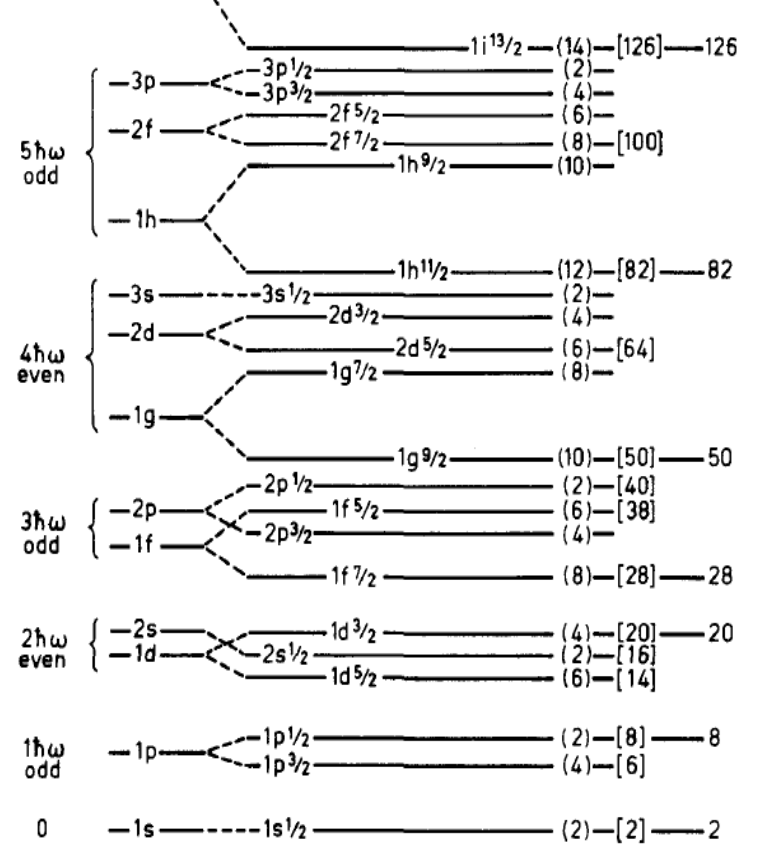
\includegraphics[width=0.7\textwidth]{figures/nuclear_shells.png}
    \caption{One-particle orbits}
    \label{fig:shell-orbits}
\end{figure}

\section{Collective model}

It is used to describe the vibrations of the nucleus.
In full generality, the angular distribution of the radius will look like

\begin{equation}
    R (\theta, \varphi) = R_0 \qty(1 + \sum _{l=0}   ^{\infty} \sum _{m=-l}   ^{l} \alpha_{lm} Y_{lm} (\theta, \varphi))
\end{equation}

where the \(Y_{lm}\) are the normalized spherical harmonics (functions \(Y: S^2 \rightarrow \C\) which satisfy \(\nabla^2 Y = 0\), \(L^2 Y_{lm} = \hbar^2 l (l+1)\), \(L_z Y_{lm} = \hbar m\)).

The term \(\alpha_{00}\) is only relevant at very high energies (it is spherically symmetrical compression/expansion). The term \(\alpha_{1m}\) correspond to translation, not an intrinsic vibration. So, we look at the quadrupole term, \(\alpha_{2m}\).

We can perform a rotation \(\alpha_{2 \mu} \rightarrow a _{2 \mu} \) using the Wigner matrices\footnote{They are the matrix elements of rotations with respect to the harmonics:
\begin{equation}
    \mathcal D^j_{mm'}(\alpha, \beta, \gamma) = \bra{jm'} \exp(-i \alpha J_z) \exp(-i \beta J_y) \exp(-i \gamma J_z) \ket{jm}
\end{equation}
}
to go into a frame where \(a_{21} = a_{2(-1)} = 0\) and \(a_{22} = a_{2(-2)}\). We parametrize the nonzero \(a\)s as \(a_{20} = \beta \cos(\gamma) \), \(a_{2(\pm 2} = \beta \sin(\gamma) / \sqrt{2}\). We used up 3 of the 5 dimensions for this.

The parameter \(\beta = \sum  \abs{a_{2m}}^2  \) describes the magnitude of the deformation, the parameter \(\gamma\) describes its direction: it can be shown that

\begin{equation}
    R_k = R_0 \qty(1+\frac{5}{4 \pi} \beta \cos(\gamma + \frac{2}{3} \pi k) )
\end{equation}

where \(k = 1, 2, 3\).

We write the Hamiltonian of the oscillation with respect to the parameters \(\alpha_{2\mu}\): the corresponding momenta are \(\pdv*{}{\alpha_{2\mu}} = \pi_{2\mu}\). Modelling the low-energy vibrations as a harmonic oscillator we get

\begin{equation} \label{eq:collective-oscillation-hamiltonian}
    H = \frac{\pi_{2\mu} \pi_{2\mu}^\dag}{2B} + \frac{C}{2} \alpha_{2\mu} \alpha_{2\mu}^\dag
\end{equation}

and we have expressions for \(B, C\).

The solutions for the Hamiltonian \eqref{eq:collective-oscillation-hamiltonian} can be shown to have energy \(E = (\sum_\mu n_\mu + 5/2) \hbar \omega\), with \(\omega = \sqrt{C/B}\). This formula implies the presence of degeneracy, but this is partially removed when introducing perturbations.

We can express the energy quantum number wrt the parameters \(\beta\) and \(\gamma\): \(\sum _{\mu}  n_\mu = 2n_\beta + \tau \), where \(\tau (\tau+3)\) is the eigenvalue of the Casimir operator on \(SO(5)\).

\section{\(\alpha\) decay}

\(\alpha\) particles are \(^{4} \ce{He} \) nuclei. That configuration has a particularly high binding energy per nucleon. The reaction in \(\alpha\) decay looks like

\begin{equation}
    ^{A} _Z X \rightarrow ^{A-4} _{Z-2} Y + \alpha
\end{equation}

For it to happen, we must have \(M(A, Z) > M(A-4, Z) + M(4, 2)\). We can expand this in terms of the binding energies, and see that it will happen only for nuclei for which \(B/A\) is decreasing with \(A\). The difference in energy between \(X\) and \(Y + \alpha\) is denoted as \(Q\). Since the velocities are not relativistic, the energy can be written as \(Q = p_\alpha^2 /2m_\alpha + p_Y^2 /2m_Y\), and since \(m_\alpha \ll m_Y\) but \(\abs{p_\alpha} = \abs{p_Y}\) the energy is almost all kept by the \(\alpha\).

Different decays have wildly different half-lives: the empirical law they follow is called the \emph{Geiger-Nuttal} \eqref{eq:geiger-nuttal}. It is very closely followed if we fix an even \(Z\) and vary \(N\) keeping it even as well.

\begin{equation} \label{eq:geiger-nuttal}
    \log(t_{1/2} ) \propto Q^{-1/2}
\end{equation}

This can be understood with quantum tunneling. First of all, we assume the \(\alpha\) can be spontaneously formed inside the nucleus as a cluster since it is a stable configuration, with some probability \(\P _ \text{formation} = \abs{\bra{\psi(A, Z)} \qty(\ket{\psi(A-4, Z-2)} \otimes \ket{\psi(4, 2)})}^2 \).

Then, this \(\alpha\) will collide with the nucleus border at some rate, which we estimate as \(f = 2 r / v\). A very rough estimate gives \(1/f \sim \hbar/\SI{}{MeV} \approx \SI{200}{MeVfm}/ (c\SI{}{MeV}) \approx \SI{e-21}{s} \).

So, we have to understand what happens at the nucleus border. We model the potential as a well, flat inside the nuclear radius \(R\); outside, the \(\alpha\) will feel the Coulomb repulsion of the nucleus

\begin{equation}
    V(r) = \frac{e^2}{4 \pi \varepsilon_0} \frac{Z_Y Z_\alpha}{r} [r \geq R] - V_0 [0 \leq r < R]
\end{equation}

Where \([\cdot]\) is the Iverson bracket.

The \(\alpha\) can tunnel through the potential barrier: how likely is it to do so? Let us call this probability \(T\). We can calculate it modelling our potential as many infinitesimal rectangular slices, let us also call \(r=b\) the point at which \(V(r) = Q\). Then,

\begin{equation}
    T = \exp(-2 \int _{R}   ^{b} \sqrt{\frac{2m(V(r) - Q)}{\hbar^2}}  \dd{r}  )
\end{equation}

since we know the wavefunction to be exponentially depressed as \(\exp(-\Delta r \sqrt{2m(V-Q)/\hbar^2} ) \) for a constant \(V>Q\) and finite \(\Delta r\), so we make \(\Delta r\) small and then we multiply together all the infinitesimal exponential probability decreases. The factor 2 comes from the fact that, to get the probabilities, we must take the square modulus.

This can be analytically calculated: if \(T = \exp(-2G) \), then

\begin{equation}
G = 2 \frac{Ze^2}{\hbar c} \sqrt{\frac{2m_\alpha c^2}{Q}}
\qty(\arccos(\sqrt{\frac{Q}{B}} ) - \sqrt{\qty(\frac{Q}{B}) \qty(1 - \frac{Q}{B})} )
\end{equation}

In the end, we can calculate the rate of decay as \(\lambda = \P _ \text{formation} T f\). As always, the decay law is \(N(t) = N_0 \exp(-\lambda t) \).

The orders of magnitude at play are as follows: \(\P _{\text{formation}} \sim 1 \), \(f \sim \SI{e21}{Hz} \), \(G \sim 30 \divisionsymbol 50\).

\section{\(\beta\) decay}

A nucleon has its isospin flipped, emitting a \(e^{\pm}\) and an electronic (anti)neutrino. This type of decay is due to the weak interaction.

Since it is a three-body process, we get a continuous spectrum of energies for the electron/positron.

\paragraph{Fermi theory}

Our assumptions are:

\begin{enumerate}
    \item we neclect the Coulomb interaction between the electron and the nucleus (this will have to be reconsidered, since it only gives accurate predictions for \(Z<10\));
    \item we neglect the recoil of the nucleus after the decay (the mass differences are very large: this will always work);
    \item we assume \(m_\nu = 0\); \label{item:beta-null-mass-assumption}
    \item we assume the distribution of energy partitions between the electron and neutrino to be uniform.
\end{enumerate}

\paragraph{Fermi's golden rule}

The rate \(\lambda\) of a transition is given by

\begin{equation} \label{eq:beta-fermi-golden-rule}
    \lambda = \frac{2 \pi}{\hbar} \abs{M}^2 \dv{n}{E}
\end{equation}

where \(M = \bra{\psi_f} H \ket{\psi_i}  \) is the matrix element between the initial and final states, \(H\) being the Hamiltonian due to which the transition happpens, \(\dv*{n}{E} \) is the differential phase volume corresponding to the energy \(E\).
Note that \(H\) is dimensional, it is an energy!

% this is trivial in retrospect but I spent some time
% assuming M was adimensional trying to figure out the
% dimensionality of this formula...

\paragraph{State density}

Recall the momentum dependence of the density of states from equation \eqref{eq:fermi-model-momentum-density}. Then

\begin{equation}
    \dd{n} = \qty(\frac{4 \pi V}{h})^3 p^2_e \dd{p_e} p^2_\nu \dd{p_\nu}
\end{equation}

The total energy is \(E_0 = E_e + E_\nu\). We work at a fixed electron energy and momentum: so because of condition \ref{item:beta-null-mass-assumption}, \(E_\nu = p_\nu c\), therefore \(\dd{p_\nu}  = \dd{E_0} /c\) and \(p_\nu^2 = (E_0 - E_e)^2/c^2\).
%Also, \(E_e = T_e + m_e c^2\).
So we get

\begin{equation}
    \dd{n} = \qty(\frac{4 \pi V}{h})^3 \frac{\dd{E_0}}{c} \frac{(E_0 - E_e)^2}{c^2} p^2_e \dd{p_e}
\end{equation}

\paragraph{Calculation of \(\lambda\)}

We can plug this (with the \(\dd{E_0}\) brought to the left hand side) into equation \eqref{eq:beta-fermi-golden-rule}, but we still have a differential to the right and we fixed \(p_e\), so we will not obtain \(\lambda\) but the \(\dd{\lambda}\) from this momentum to \(p_e + \dd{p_e} \).

\begin{equation} \label{eq:beta-diff-lambda}
    \dd{\lambda}
    = \frac{2 \pi}{\hbar} \abs{M}^2  \qty(\frac{4 \pi V}{h})^3 F(Z_Y, E_e) \frac{(E_0 - E_e)^2}{c^3} p^2_e \dd{p_e}
    =  \abs{M}^2  \frac{(4 \pi V)^3}{c^3 h^4} F(Z_Y, E_e) (E_0 - E_e)^2 p^2_e \dd{p_e}
\end{equation}

We get \(\lambda\) by integrating this expression. We also added a factor to account for the asymmetry between electrons and positrons: the former are slowed down by electrostatic attraction when leaving the nucleus, the latter are accelerated. So, we multiply \(\lambda\) by \(F(Z_Y, E_e) = 2 \pi \eta / (1- \exp(-2 \pi \eta ))\), %\footnote{\(\approx \eta/2+1\) when \(\eta \approx 0\)}
where \(\eta = \mp \alpha Z_Y / \beta_e\), \(\alpha\) being the fine-structure constant.

\begin{equation}\label{eq:beta-int-lambda}
    \lambda = \abs{M}^2  \frac{(4 \pi V)^3}{c^3 h^4} F(Z_Y, E_e) \int (E_0 - E_e)^2 p^2_e \qty[0 \leq (p_e c)^2 \leq E_0^2 - m_e^2 c^4] \dd{p_e}
\end{equation}

\paragraph{Fermi-Kurie plot}

Flipping equation \eqref{eq:beta-diff-lambda} around, we find that

\begin{equation}
    K(E_e) = \sqrt{ \dv{\lambda}{p_e} F^{-1} p_e^{-2} } \propto E_0 - E_e
\end{equation}

a testable prediction, which is experimentally verified. Sometimes we get sums of different lines (in the limit in which the \(K\)s are additive? maybe we can say that the \(\dd{\lambda} \)s are additive and small so we make it work...).

If we had \(m_\nu \neq 0\), the \(K\) plot would no longer be linear in \(E_e\) (instead of \(p_\nu^2 = (E_0 - E_e)^2/c^2\) we would have had \(p_\nu^2 = (E_0 - E_e) \sqrt{(E_0-E_e)^2 - m_\nu ^2 c^4} /c^2\)). This allows us to measure the neutrino mass.

From equation \eqref{eq:beta-int-lambda} we can calculate \(ft \defeq F(Z_Y, E_e) \log(2) / \lambda \). This is known as the \(ft\) value: it gives an estimate of \(\abs{M}^{-2} \). We usually plot its base-10 logarithm, since it varies through many orders of magnitude.

\paragraph{Calculating the matrix element}

We assume the interaction Hamiltonian is in the form \(H = g \delta^3(r_e-r) \delta^3(r_\nu - r)\). In the calculation of \(M\) this will make all the integrals in the same variable, \(r\).
\(g\)'s value cannot be determined theoretically, experimentally \(g \approx \SI{e-4}{MeV fm^{3}} \).
We must evaluate an expression as follows:

\begin{equation}
    M = \int  \psi_\nu^* \psi_e^* \psi_{\text{nuc - f}}^* \psi_{\text{nuc - i}}  \dd{r}
\end{equation}

where all the wavefunctions are evaluated at \(r\). If the electron and neutrino wavefunctions are planar waves, say \(\psi_e = \exp(-ipr/\hbar) \sim 1 - ipr/\hbar + o(r)\). But we integrate only over the support of the nuclear wavefunctions: let us assume \(r = r_0 A^{1/3} \approx 3 \divisionsymbol 5\) and \(p = \sqrt{E_e^2/c^2 - m_e^2 c^2} \approx \SI{1}{MeV/c}  \). Then we see that the first order term is negligible. We do this for the electron and neutrino, getting
\(M = g \braket{\text{nuc - f}}{\text{nuc - i}}/V \), where \(V\) is the volume we assume the electron and neutrino wavefunctions are normalized to have support in.

This is equivalent to assuming \(p \wedge r = L = 0\) for the electron and neutrino.

\paragraph{Transition types}

We call the nuclear angular momentum \(I\), the leptons' total angular momentum and spin \(L\) and \(S\). Then

\begin{equation}
    \vec{I_i} = \vec{I_f} + \vec{L} + \vec{S}
\end{equation}

we distinguish

\begin{enumerate}
     \item Fermi transitions: \(S = 0\).
    \item Gamow-Teller transitions: \(S = 1\).
\end{enumerate}

\begin{enumerate}
    \item Permitted transitions: \(\Delta L =0\), they also have no change in parity since \(\Delta \pi = (-)^{\Delta L}\). They are the ones we described in the last paragraph.
    \item Super-permitted transitions: the starting and ending nuclear configurations are almost identical. This happens with specular nuclei. \(\log_{10}(ft) \sim 3.5 \).
    \item Prohibited transitions (of various orders): every additional term in the expansion of the lepton wavefunctions depresses \(\abs{M}^{2} \) by a factor \SI{e4}{}, so they get increasingly unlikely.
\end{enumerate}

\section{\(\gamma \) decay}

\(\gamma\) radiation is almost monochromatic, since excited states usually live for around \(\SI{e-12}{s} \approx 1/ \SI{6.6e-4}{eV} \); its wavelength is also much longer than the nucleus.

The energy lost from the excited state is almost all with the \(\gamma\): if we assume that energy and momentum are conserved we get \(\Delta E = E_\gamma - E_\gamma^2 / (2M)\) since \(E_\gamma = p_{\text{recoil}}\). The solution of this is:

\begin{equation}
    E_\gamma = M \qty(-1 \pm \sqrt{1+ \frac{\Delta E}{M}} ) \approx \Delta E - \frac{\Delta E ^2}{M} \approx \Delta E
\end{equation}

\paragraph{Selection rules}

We must have \(\vec{I_i} = \vec{I_f} + \vec{L} \), and the angular momentum of the photon must be nonzero. Also, let us call \(EL\) the electric (due to moving charge) radiation with momentum \(L\) and \(ML\) the analogous magnetic (due to moving current) radiation. We call it \(2^L\)-pole radiation. Then it can be shown that

\begin{equation}
    EL \iff \Delta \pi = (-)^L \qquad
    ML \iff \Delta \pi = (-)^{L+1}
\end{equation}

\paragraph{Emitted power}

Let us compare the emitted power to the first order of an electric dipole \(d\) vs a magnetic dipole \(\mu\), using the EM-fields formulas: \(P(E1) \sim \omega^4 d^2 / c^3\), while \(P(M1) \sim \omega^4 \mu^2 / c^5\). In general, denoting \(\sigma = E, M\):

\begin{equation}
    P(\sigma L) = \frac{2c}{\varepsilon_0} \frac{(L+1)}{L((2L+1)!!)^2} \qty(\frac{\omega}{c})^{2L+2} \mathcal M (\sigma L)^2
\end{equation}

where \(\mathcal M\) can be interpreted, in a quantum setting, as a \emph{transition amplitude}, whose square modulus is a transition probability.
To calculate \(\mathcal M\) we should use the multipole operators, which for the electric transitions are \(O(EL) = e r^L_i Y_{i,LM}\) (\(i\) labels the particles in the nucleus) while the magnetic ones are much more complicated.

In general, \(\mathcal M (\sigma L) = \bra{\psi_f} O(\sigma L) \ket{\psi_i} \).
Dimensionally, \([\mathcal M] = C m^L\).

We can find the rate of photon emission as \(T(\sigma L) = P(\sigma L) / \hbar \omega\).

\begin{equation}
    T(\sigma L ) =
    \frac{8 \pi \alpha c (L+1)}{e^2 L (2L+1)!!^2} \qty(\frac{\omega }{c})^{2L+1}
    \abs{\mathcal M (\sigma L)}^2
\end{equation}

\paragraph{Weisskopf estimations}

Instead of the multipole operators, we use brutal estimates (the radial wavefunctions are proportional to \([r \in \text{nucleus}]\), the angular integrals are 1):

\begin{subequations}
\begin{align}
    \abs{\mathcal M (EL)}^2/e^2 &= \frac{1}{4 \pi} \qty(\frac{3}{3+L}) ^2 (r_0 A^{1/3})^{2L} \\
    \abs{\mathcal M (ML)}^2 &\propto \qty(\frac{3}{3+L}) ^2 (r_0 A^{1/3})^{2L-2}
\end{align}
\end{subequations}

The ratio of the magnetic to electric matrix square element is something like \(0.31A^{-2/3} \sim \SI{e-2}{} \). The take-away is: when \(L\) increases by 1, the transition probability decreases by a factor \(\SI{e4}{} \divisionsymbol \SI{e5}{} \).

In the end, setting \(R = r_0 A^{1/3}\), we get

\begin{equation}
    T(E L ) \approx
    \frac{2 \alpha (L+1)}{L (2L+1)!!^2} \qty(\frac{\omega}{c})^{2L+1} \qty(\frac{3}{3+L})^2 R^{2L}
\end{equation}

Around magic numbers this prediction is close to being verified; mid-shell we see tens or hundreds more than it. The half-life of the decay is given by \(t_{1/2} = \log(2)/T  \)

\paragraph{Experimental methods}

We can experimentally determine the parity of a \(\Gamma\) transition: we look at the differential cross section \(\dv*{\sigma}{\theta} \) wrt the azimuth angle \(\theta\), if it is odd then the change in parity is \((-)\), if it is even the change in parity is \((+)\).

Also, we can look at the number of nodes \(\dv*{\sigma}{\theta} \), which will be equal to the order of the Legendre polynomial of the radiation.

\section{Matter and radiation}

\paragraph{Cross sections}

The flux of particles \(\varphi = \# \text{particles} / (A t)\) decays like \(\Delta \varphi = - \varphi \sigma n_t \Delta x\), where \(n_t\) is the particle density in the target, and the proportionality constant \(\sigma\) \([\SI{}{m^2} ]\) is called the scattering cross section.

\paragraph{Photons}

\textbf{Photoelectric}: \(\sigma \sim Z^{4 \divisionsymbol 5} / E_\gamma^3\),
for \(E _\gamma < \SI{400}{keV} \).

\textbf{Compton}: continuous spectrum,

\begin{equation}
    E _ \gamma '  = \frac{E_ \gamma}{1 + (E_\gamma / m_e c^2) (1- \cos(\theta))}
\end{equation}

The maximum energy transferred to the electron is at \(\theta \rightarrow \pi\), \(E_ \gamma ' - E_ \gamma \rightarrow m_e c^2/2\).

\textbf{Pair production} Near a nucleus, we can have some momentum transfer and see \(\gamma \rightarrow
e^- + e^+\).

\paragraph{Bethe-Bloch}


\end{document}
